\documentclass[twocolumn,oneside]{article}
\usepackage{Pseudopotenciales}

\title{\vspace{-2cm}{\LARGE {\bf Universidad Nacional Aut\'onoma de M\'exico}}\\ 
{\large Tesis: C\'alculos Cu\'anticos de Hidrataci\'on de Lant\'anidos}\\
\vspace{0cm}
Metodolog\'ia: Pseudopotenciales\\ 
\vspace{0cm}}
\author{
Braulio Joel Rojas Mayoral\vspace{0cm}} 
\date{{\small Diciembre de 2012}}
\makeindex
\begin{document}
\hyphenation{
% a
a-lea-to-ria-men-te
% b
% c
ca-rac-te-ris-ti-cas
cons-truir
cons-tru-y\'o
co-rres-pon-de
cua-li-ta-ti-vas
% d
des-crip-ci\'on
di-fe-ren-cias
% e
e-li-mi-nar
e-ner-g\'i-a
% f
fa-mi-lia-res
% g
ge-ne-ra-ci\'on
ge-ne-ra-dos
% h
ha-mil-to-nia-no
hi-dra-ta-ci\'on
% i
% j
% k
% l
li-neal
% m
mo-le-cu-la-res
% n
% o
ob-te-ner
% p
pa-r\'a-me-tros
pro-ba-bi-li-dad
pro-ble-mas
% q
% r
% s
% t
% u
% v
% w
% x
% y
% z 
}

\maketitle
\pagenumbering{roman}
%\tableofcontents
\renewcommand\tablename{Tabla}
%\listoftables

%{\normalsize
%\input{agradecimiento.tex}
%\newpage}

%{\normalsize
%\input{dicatoria.tex}
%\newpage}

%{\normalsize
%\input{resumen.tex}
%\newpage}



%\linespread{1.75}
\setcounter{page}{1}
\pagenumbering{arabic}
{\normalsize
\subsection{Pseudopotenciales}
%DolgChemRev2012.112.403
%\paragraph{Electrones de valencia y de carozo}
Los conceptos de valencia y electrones de carozo son familiares para
todo qu\'imico y fundamental, por ejemplo, para el ordenamiento de 
los elementos en la tabla peri\'odica. Para muchas consideraciones
cualitativas la qu\'imica de un elemento es solo determinada por sus
electrones de valencia, los cuales participan activamente en los 
enlaces qu\'imicos. En esta descripci\'on los electrones de carozo 
permanecen esencialmente sin participaci\'on y a lo m\'as juegan un 
rol indirecto, por ejemplo, proporcionando junto con el n\'ucleo un 
potencial efectivo modificado para los electrones de valencia dentro
de un grupo de la tabla peri\'odica. Las modificaciones en los 
potencial efectivo no solo llevan a diferencias cuantitativas para 
los \'atomos, por ejemplo, en los potenciales de ionizaci\'on, 
afinidad electr\'onica y energ\'ias de excitaci\'on, sino tambi\'en 
para mol\'eculas, por ejemplo, las fuerzas en los enlaces qu\'imicos 
formados por estos \'atomos, y as\'i afectando su comportamiento 
qu\'imico \citep{Dolg2012}.

%\paragraph{Potenciales Efectivos de Carozo}
El m\'etodo de potenciales efectivos de carozo (ECPs, por sus siglas 
en ingl\'es) hace uso de estas ideas en los c\'alculos te\'oricos de 
la estructura electr\'onica a primeros principios. Las principales 
finalidades son una considerable reducci\'on del esfuerzo 
computacional evitando el costoso tratamiento expl\'icito de los 
carozos at\'omicos en los c\'alculos y al mismo tiempo un tratamiento
impl\'icito de la mayor\'ia de los efectos relativistas para el 
sistema de electrones de valencia. La eliminaci\'on de los carozos
at\'omicos de los c\'alculos permite tratar todos los elementos de un
grupo de la tabla peri\'odica de igual manera. Ya que el mismo 
n\'umero de electrones de valencia deben de ser tratados para todos
los elementos de una columna de la tabla peri\'odica, se espera que
el mismo esfuerzo computacional y una precisi\'on similar sea lograda,
es decir, la variaci\'on en la calidad de los resultados causada por la 
gran diferencia en el tama\~no de los sistemas es evitada. 
Claramente, tal expectaci\'on descansa en la suposici\'on discutible 
de que el formalismo de los ECPs trabaja igualmente bien para todos los 
elementos de un grupo de la tabla peri\'odica. 

%\paragraph{Efectos Relativistas}
Los efectos relativistas para los elementos pesados no pueden ser 
ignorados ya que provocan cambios cuantitativos e incluso a veces 
cualitativa a la precisi\'on de la investigaci\'on. Estas
contribuciones relativistas requieren un esfuerzo computacional 
adicional a en c\'alculos de todos los electrones (AE, por sus siglas
en ingl\'es). Dentro de la descripci\'on ECP ellas son usualmente 
incluidas por medio de una simple parametrizaci\'on del hamiltoniano 
modelo solo de valencia elegido con respecto a datos de referencia 
relativistas de AE. La descripci\'on ECP escalar relativista puede 
hacer uso de toda la maquinaria sin cambio de la qu\'imica cu\'antica
no-relativista cuando los efectos esp\'in-\'orbita pueden ser 
ignorados, sin embargo logrando resultados comparables a aquellos 
c\'alculos de mayor costo, escalar relativista de AE. Los efectos SO 
pueden ser tomados en cuenta en una descripci\'on ECP usando varias 
estrategias, por ejemplo, un tratamiento perturbativo subsecuentes a
los c\'alculos escalares relativistas, esto es, como el \'ultimo paso
del c\'alculo, o para su rigurosa inclusi\'on variacional desde el 
comienzo de los c\'alculos. Que los ECPs se vuelven un caballo de 
batalla de la qu\'imica cu\'antica relativista no es sorprendente, 
esto se debe que los resultados obtenidos en la mayor\'ia de las 
investigaciones de problemas qu\'imicos por los modernos esquemas ECP
son tan precisos como aquellos obtenidos de los m\'as costosos, y
tambi\'en aproximados c\'alculos relativistas AE, por lo que producen
m\'as resultados que ning\'un otro m\'etodo relativista. 

%\paragraph{Nomenclatura de potenciales efectivos de carozo}
Los potenciales modelos intentan construir potenciales efectivos
anal\'iticos modelando directamente el potencial HF no local original
para los electrones en orbitales de valencia los cuales tienen la 
estructura nodal completa de los orbitales de valencia AE. Esto se
logra haciendo uso de la ecuaci\'on de Huzinaga-Cantu y ser\'a 
referida como una descripci\'on de potenciales modelos HF (MP). 
Hay otro m\'etodo para la descripci\'on de Pseudopotenciales que 
modelan el potencial no local HF usando orbitales de pseudovalencia, 
esto es, orbitales que despu\'es de una transformaci\'on aun den las 
energ\'ias orbitales correctas, pero tienen una estructura nodal 
radial simplificada. Este m\'etodo se basa en la ecuaci\'on de 
Phillips-Kleinman y ser\'a referido como la descripci\'on de 
pseudopotenciales modelos HF (PP).

%\paragraph{Aproximaciones Pr\'acticas}%pag 417
Algunas aproximaciones deben de ser hechas para lograr un esquema 
pr\'actico computacionalmente de los c\'alculos de Orbitales de 
Valencia. Primero se deben de separar los sistemas en electrones de 
valencia y los de carozo. Segundo, se debe suponer que los carozos 
at\'omicos est\'an inertes y se mantienen sin cambio cuando van de un
sistema a otro. Tercero, para eliminar los electrones de carozo y 
posiblemente tambi\'en los orbitales internos de los c\'alculos se 
debe reemplazar su contribuci\'on en un hamiltoniano de AE a los 
electrones de valencia por un potencial efectivo de carozo modelando 
el potencial HF no local real. Y cuarto, los m\'etodo ECP casi 
siempre asumen que los carozos at\'omicos no interaccionan con los 
carozos de otros \'atomos excepto por su repulsi\'on coulombiana.

{\normalsize
\subsection*{Base de \cite{Yang2005}}
%\paragraph{Orbital de Cristal}
%Esta informaci\'on fue tomada de old.iupac.org
Orbital de cristal (sin\'onimo banda orbital), es la funci\'on de un
electr\'on extendida a trav\'es de un cristal. T\'ipicamente una 
combinaci\'on lineal de orbitales de Bloch:
$$\Psi_j=\sum_{\mu}a_{j\mu}\phi_{\mu}.$$
Los orbitales de Bloch incorporan la simetr\'ia de translaci\'on
aplicando condiciones a la frontera
$$\phi_{\mu}(\vec r)=\sum_n\exp{ikr}\chi_{\mu}(\vec r)$$
donde $\chi_{\mu}(\vec r)$ es el n-\'esimo orbital at\'omico definido 
el vector de translaci\'on $\vec r$. Los diferentes valores adoptados
por el vector de onda $\vec k$ determinan la simetr\'ia y las 
propiedades nodales del orbital de cristal.

%\paragraph{?`Porqu\'e orbitales de cristal}
%YangTheorChemAcc2005.113.212
Gracias a los recientes logros en la descripci\'on y predicci\'on las
propiedades de bulto de los materiales, los c\'alculos de las 
estructuras electr\'onicas se han vuelto m\'as importantes tanto en
qu\'imica como en f\'isica de materia condensada para dise\~nar y 
preparar materiales con propiedades controladas. El acceso a 
c\'odigos complicados y poder de c\'omputo ha hecho posible 
experimentos computacionales {\it ab initio}. Estos c\'alculos de 
primeros principios fueron hechos com\'unmente usando bases de ondas 
planas junto con Pseudopotenciales y teor\'ia del funcional de la 
densidad en f\'isica del estado s\'olido. Los m\'etodos de Orbitales 
de Cristales gan\'o atenci\'on en el c\'alculo de s\'olidos desde la
implementaci\'on de la combinaci\'on lineal de orbitales at\'omicos 
Hartree-Fock (LCAO) en el programa CRYSTAL para el tratamiento de 
sistemas peri\'odicos. Los m\'etodos de ECP han sido aplicados a los 
lant\'anidos principalmente para eliminar la capa abierta 4f y los
principales problemas relacionados a esta. %(?`Cu\'ales son esos problemas?). 
Sin embargo, los conjuntos de valencia generados para pseudopotenciales 
consistentes con la energ\'ia de los lant\'anidos para aplicaciones
moleculares no pueden ser transferidos directamente a componentes 
peri\'odicos sin modificaci\'on. La raz\'on es que, frecuentemente,
los conjunto de bases at\'omicas con funciones difusas dan como 
resultado un traslape entre funciones de Bloch que construyen los 
orbitales de cristal y as\'i no solo dan como resultado un 
desperdicio de recursos computacionales sino que adem\'as pueden 
causar problemas con dependencia cuasilineal debido a las 
limitaciones num\'ericas. 

%\paragraph{Resumen del trabajo de \cite{Yang2005}}
\cite{Yang2005} optimizaron un conjunto de bases Gaussianas a la 
energ\'ia HF para toda la serie de los iones de lant\'anidos
trivalentes (desde lantano hasta lutecio), adem\'as las derivaron y 
adaptaron para c\'alculos de Orbitales de Cristal usando los 
pseudopotenciales de Stuttgart-Koel de consistencia energ\'etica. 

%\ocultartrue
%\begin{Vocultar}
%\paragraph{Breve Teor\'ia de los OC}
%La naturaleza de los orbitales de cristal $\psi_i(r;k)$ en sistemas 
%peri\'odicos, los cuales son una combinaci\'on lineal de funciones de
%Bloch $\phi_{\mu}(r;k)$ que son contraidas a funciones gaussianas 
%(\ref{OC}). Cada funci\'on de Bloch es definida como la suma de los 
%mismos orbitales at\'omicos (OA,$\varphi_{\mu}(r-A_{\mu}-g)$) 
%trasladados sobre un enrejado infinito con cada OA multiplicado por 
%una onda plana (\ref{FB}), las cuales son expresadas como una 
%combinaci\'on lineal funciones gaussianas generadas (\ref{FG}). 
%As\'i, el conjunto de bases real son las funciones de Bloch debido a
%la raz\'on los coeficientes de combinaci\'on $a_{\mu,i}$ est\'an 
%involucrados en el procedimiento variasional y contribuyen en los
%c\'alculos de los elementos de la matriz densidad. Ya que el esquema
%es conservado, la libertad variasional es constante, y las funciones
%de Bloch no son sensibles al aumento en el tama\~no de las funciones
%primitivas de (4s4p3d) a (6s6p5d) debido al t\'ermino de las ondas
%planas $\exp{ik\cdot g}$, aunque un aumento en el n\'umero de 
%primitivas proporciona una mejor descripci\'on de OA.
%
%\be\label{OC}
%\psi_i(r;k)=\sum_{\mu}a_{\mu,i}(k)\phi_{\mu}(r;k)
%\ee
%\be\label{FB}
%\phi_{\mu}(r;k)=\sum_{g}\varphi_{\mu}(r-A_{\mu}-g)\exp{ik\cdot g}
%\ee
%\be\label{FG}
%\varphi_{\mu}(r-A_{\mu}-g)=\sum^{n_G}_{j}d_jG(\alpha_j;r-A_{\mu}-g).
%\ee
%\end{Vocultar}
}

}
%\newpage}

%{\normalsize
%\input{objetivos.tex}}
%\newpage}

%{\normalsize
%\input{metodologia.tex}}
%\newpage}

%{\normalsize
%\documentclass[onecolumn,oneside]{article}
\usepackage{Resultados}

\title{\vspace{-2cm}{\LARGE {\bf Universidad Nacional Aut\'onoma de M\'exico}}\\ 
{\large Seminario de Tesis}\\
\vspace{0cm}
Resultados\\ 
\vspace{0cm}}
\author{
Braulio Joel Rojas Mayoral\vspace{0cm}} 
\date{{\small Abril de 2013}}
\makeindex
\begin{document}
\hyphenation{
% a
a-lea-to-ria-men-te
% b
% c
ca-rac-te-ris-ti-cas
cons-truir
cons-tru-y\'o
co-rres-pon-de
cua-li-ta-ti-vas
% d
des-crip-ci\'on
di-fe-ren-cias
% e
e-li-mi-nar
e-ner-g\'i-a
% f
fa-mi-lia-res
% g
ge-ne-ra-ci\'on
ge-ne-ra-dos
% h
ha-mil-to-nia-no
hi-dra-ta-ci\'on
% i
% j
% k
% l
li-neal
% m
mo-le-cu-la-res
% n
% o
ob-te-ner
% p
pa-r\'a-me-tros
pro-ba-bi-li-dad
pro-ble-mas
% q
% r
% s
% t
% u
% v
% w
% x
% y
% z 
}

\maketitle
\pagenumbering{roman}
%\tableofcontents
\renewcommand\tablename{Tabla}
%\listoftables

\setcounter{page}{1}
\pagenumbering{arabic}

{\normalsize
\section{Informaci\'on Geom\'etrica}
%\paragraph{Geometr\'ia} 
Es muy bien aceptado que el n\'umero de
coordinaci\'on (NC) de los lant\'anidos trivalentes cambia a lo largo
del periodo 4f, teniendo un NC=9 para los primeros Ln(III), mientras
un equilibrio es establecido entre NC=8 y NC=9 en los elementos de la
mitad de la serie, los \'ultimos tienen un NC=8. Teniendo lo anterior
en cuenta dos gr\'aficas de las distancias promedios te\'oricas de 
los lant\'anidos a los ox\'igenos, en sistemas con coordinaci\'on 8 y 
9, as\'i como de los datos experimentales son mostradas en las figuras 
\ref{fDLO2} y \ref{fDLO3}, en donde los lant\'anidos de la mitad de la
serie son repetidos en las dos gr\'aficas, Eu-Tb, y en la tabla 
\ref{tDis} los valores son presentados. 

%\paragraph{Simbolog\'ia}
Los resultados fueron 
obtenidos con diferentes pseudopotenciales, diferentes bases para el
mismo pseudopotencial y a diferentes niveles de c\'alculo y utilizando
teor\'ia de perturbaciones M\o ller-Plesset y la correcci\'on SCS 
\citep{Grim2003}. Los c\'alculos con diferentes pseudopotenciales son
identificados con diferentes figuritas, $\clubsuit$ corresponde a la
utilizaci\'on del pseudopotencial largo \citep{Dolg1989} y 
$\spadesuit$ corresponde al pseudopotencial corto \citep{Cao2001}. 
Las bases son representadas por n\'umeros, del 1 al 3, 1 corresponde 
a la base corregida de \cite{Dolg1993}, 2 la base extendida de 
\cite{Yang2005} y 3 corresponde a la base segmentada de 
\cite{Cao2002}. El n\'umero 4 representa c\'alculos utilizando la
correcci\'on de \cite{Grim2003} al m\'etodo MP2 adem\'as de agragar
los efectos de bulto. Finalmente a los datos experimentales se les
identifica con el n\'umero 5.
% y presentada en la tabla \ref{tDLO}

%\paragraph{Figura \ref{fDLO2}}
La figura \ref{fDLO2} corresponde a las distancias promedio
ox\'igeno-lant\'anido, para sistemas con n\'umero de coordinaci\'on 
nueve. Los resultados obtenidos a nivel MP2 utilizando el 
psuedopotencial largo \citep{Dolg1989} y su base corregida 
\citep{Dolg1993} reproducen la tendencia, tri\'angulos 
negros en la gr\'afica, pero la distancia es mayor a la experimental,
cruces rojas. Por ejemplo, para el lantano se obtiene una distancia de
2.6196 \AA, mientras que el valor experimental reportado es 2.600 \AA.
En cambio, utilizando la base extendida \citep{Yang2005} y el mismo 
pseudopotencial, tri\'angulo verde, la distancia es menor a la 
experimental, para el caso del lantano e intermedia entre la 
experimental y la te\'orica utilizando la base corregido para los 
lant\'anidos Eu-Tb. Si se cambia de pseudopotencial, al 
pseudopotencial corto \citep{Cao2001} y utilizando su base segmentada
\citep{Cao2002}, c\'irculo rojo, la distancia promedio te\'orica del 
lant\'ano a los ox\'igenos es la m\'as peque\~na, 2.5798 \AA. Si se 
utiliza el pseudopotencial largo y su base corregida, pero agregando 
los efectos de bulto, debidos a las capas de hidrataci\'on mayores, 
utilizando un modelo de medio polarizable continuo (PCM, por sus 
siglas en ingl\'es) la distancia no es tan peque\~na como la obtenida
con el pseudopotencial corto de \cite{Cao2001} ni tampoco tan grande 
como cuando no se considera los efectos de bulto utilizando la misma 
base y pseudopotencial, para el lantano se obtiene una distancia de 
2.5926 \AA. Se observa que es el resultado con la segunda diferencia 
m\'as peque\~na respecto al valor experimental, solo mayor a los 
resultados MP2$^{\clubsuit,2}$, utilizando el pseudopotencial largo y
la base extendida. Se observa que la diefencia entre las distancias
te\'oricas a nivel MP2$^{\clubsuit,1}$ y las experimentales va 
aumentando a lo largo de la serie.

%%%%%%%%%%%%%%%%%%%%%%%%%%%%%%%%%%%%%%%%%%%%%%%%%%5555
\begin{figure}[h]
\centering
\includegraphics[height=10cm,angle=-90]{Graficas/lnO9dist2.ps}
\caption{\small{Gr\'afica de la variaci\'on de la distancia promedio
lant\'anido ox\'igenoa a trav\'es de la serie 4f con n\'umero de 
coordinaci\'on igual a nueve. $^{\clubsuit}$Pseudopotencial Largo 
\citep{Dolg1989}. $^{\spadesuit}$Pseudopotencial Corto 
\citep{Cao2001}. $^1$Utilizando la base de \cite{Dolg1993}}, 
$^2$utilizando la base de \cite{Yang2005}, $^3$utilizando la base de 
\cite{Cao2002}, $^4$nivel SCS-MP2 \citep{Grim2003} y utilizando MPC 
\citep{Toma2005}, $^5$datos experimentales reportados por 
\cite{Dang2012}.}
\label{fDLO2}
\end{figure}
%%%%%%%%%%%%%%%%%%%%%%%%%%%%%%%%%%%%%%%%%%%%%%%%%%%%%%
%\paragraph{Figura \ref{fDLO3}}
La figura \ref{fDLO3} corresponde a las distancias promedio
ox\'igeno-lant\'anido, para sistemas con n\'umero de coordinaci\'on 
ocho. Los resultados obtenidos a nivel MP2 utilizando el 
psuedopotencial largo \citep{Dolg1989} y su base corregida 
\citep{Dolg1993} reproducen la tendencia, tri\'angulos 
negros en la gr\'afica, pero la distancia es mayor a la experimental,
cruces rojas. Por ejemplo, para el europio se obtiene una distancia de
2.4756 \AA, mientras que el valor experimental reportado es 2.455 \AA.
En cambio, utilizando la base extendida \citep{Yang2005} y el mismo 
pseudopotencial, tri\'angulo verde, la distancia es menor a la 
experimental, para el caso del gadolinio, e intermedia entre la 
experimental y la te\'orica utilizando la base corregido para los 
lant\'anidos Ho-Lu. Si se cambia de pseudopotencial, al 
pseudopotencial corto \citep{Cao2001} y utilizando su base segmentada
\citep{Cao2002}, c\'irculo rojo, la distancia promedio te\'orica del 
lutecio a los ox\'igenos es la m\'as peque\~na, 2.3252 \AA, mientras 
que la distancia experiemental es de 2.345 \AA. Si se utiliza el 
pseudopotencial largo y su base corregida, pero agregando los efectos
de bulto, debidos a las capas de hidrataci\'on mayores, utilizando un
modelo de medio polarizable continuo la distancia es la m\'as cercana
al dato experimental para el lutecio, se obtiene una distancia de 
2.3489 \AA. Se observa el mismo comportamiento en las diferencias 
entre las distancias te\'oricas a nivel MP2$^{\clubsuit,1}$ y las 
experimentales a las observadas en la figura \ref{fDLO2}, la 
diferencia va aumentando a lo largo de la serie de los lant\'anidos.
%%%%%%%%%%%%%%%%%%%%%%%%%%%%%%%%%%%%%%%%%%%%%%%%%%5555
\begin{figure}[h]
\centering
\includegraphics[height=10cm,angle=-90]{Graficas/lnO9dist3.ps}
\caption{\small{Gr\'afica de la variaci\'on de la distancia promedio
lant\'anido ox\'igeno a trav\'es de la serie 4f con n\'umero de 
coordinaci\'on igual a ocho. $^{\clubsuit}$Pseudopotencial Largo
\citep{Dolg1989}. $^{\spadesuit}$Pseudopotencial Corto 
\citep{Cao2001}. $^1$Utilizando la base de \cite{Dolg1993}}, 
$^2$utilizando la base de \cite{Yang2005}, $^3$utilizando la base de
\cite{Cao2002}, $^4$nivel SCS-MP2 \citep{Grim2003} y utilizando MPC 
\citep{Toma2005}, $^5$datos reportados por \cite{Dang2012}.}
\label{fDLO3}
\end{figure}
%%%%%%%%%%%%%%%%%%%%%%%%%%%%%%%%%%%%%%%%%%%%%%%%%%%%%%
%\paragraph{Las dos figuras}
En las figuras \ref{fDLO2} y \ref{fDLO3} se observa la contracci\'on 
de los lant\'anidos, cuya reproducci\'on te\'orica ya se report\'o
\citep{Kuta2010,Ciup2010,Dang2012}. Adem\'as se observa que las 
distancias promedios obtenidas a partir del pseudopotencial largo, la
base carregida y el medio polarizable continuo son menores a las 
obtenidas con el mismo pseudopotencial pero usando la base extendida.
\'Estas, a su vez, son menores a las obtenidas con el pseudopotencial
largo y su base corregida a nivel MP2, las cuales siempre fueron 
mayores a las reportadas en los experimentos y las distancias 
te\'oricas mayores. Las distancias m\'as peque\~nas se obtuvieron con
el pseudopotencial corto y siempre fueron menores a las reportadas 
experimentalmente.
  


%\paragraph{Tabla \ref{tDis}}
%%\begin{table}[h!]
\centering  %%
%\begin{center}
%\begin{table}[h!]
\caption{\footnotesize Distancias promedio del Lantano a los ox\'igenos
y los hidr\'ogenos, en {\AA}ngstr\"om.
{\footnotesize $^1$ Utilizando la base de \cite{Dolg1993}.} 
{\footnotesize $^2$ Utilizando la base de \cite{Yang2005}.}
{\footnotesize $^3$ Utilizando la base de \cite{Cao2002}.}  
{\footnotesize $^4$ Nivel SCS-MP2 \citep{Grim2003} y utilizando MPC 
\citep{Toma2005}.}}
\begin{tabular}{c|cc}\hline\hline
C\'alculo & $\overline R$(Ln-O) & $\overline R$(Ln-H) \\ \hline
HF/LCRECP & 2.6628 & 3.3244 \\ 
MP2/LCRECP$^1$ & 2.6196 & 3.3060  \\ 
MP2/LCRECP$^2$ & 2.5945 & 3.2804  \\ 
MP2/SCRECP$^3$ & 2.5798 & 3.2662  \\ 
MP2$^4$/LCRECP$^1$ & 2.5926 & 3.2793  \\ 
\hline \end{tabular}\label{tD9+0}\end{table}
%\end{center}

%%\begin{table}[h!]
\centering  %%
%\begin{center}
%\begin{table}[h!]
\caption{\footnotesize Distancias promedio del Gadolinio a los ox\'igenos
y los hidr\'ogenos, en {\AA}ngstr\"om.
{\footnotesize $^1$ Utilizando la base de \cite{Dolg1993}.} 
{\footnotesize $^2$ Utilizando la base de \cite{Yang2005}.}
{\footnotesize $^3$ Utilizando la base de \cite{Cao2002}.}  
{\footnotesize $^4$ Nivel SCS-MP2 \citep{Grim2003} y utilizando MPC 
\citep{Toma2005}.}}
\begin{tabular}{c|cc}\hline\hline
C\'alculo & $\overline R$(Ln-O) & $\overline R$(Ln-H) \\ \hline
HF/LCRECP & 2.5442 & 3.2069 \\ 
MP2/LCRECP$^1$ & 2.5028 & 3.1897  \\ 
MP2/LCRECP$^2$ & 2.4837 & 3.1701  \\ 
MP2/SCRECP$^3$ & x.xxxx & x.xxxx  \\ 
MP2$^4$/LCRECP$^1$ & 2.4785 & 3.1651  \\ 
\hline 
\multicolumn{3}{l}{\footnotesize{Esto es una mamada.}}
\end{tabular}\label{tDGd9+0}\end{table}
%\end{center}

\begin{table}[h!]
\centering  %%
%\begin{center}
%\begin{table}[h!]
\caption{\footnotesize Distancias promedio de los lant\'anidos a los 
ox\'igenos, en {\AA}ngstr\"om.}
\begin{tabular}{p{1cm}|p{1.8cm}p{1.8cm}p{1.8cm}p{1.8cm}p{1.8cm}p{1.8cm}}\hline\hline
Ion & HF$^{\clubsuit,1}$ & MP2$^{\clubsuit,1}$ & MP2$^{\clubsuit,2}$ & MP2$^{\spadesuit,3}$ & MP2$^{\clubsuit,1,4}$ & EXAFS$^5$ \\ \hline
La $^{3+}$ & 2.6628(9+0) & 2.6196(9+0) & 2.5945(9+0) & 2.5798(9+0) 
& 2.5926(9+0) & 2.600(9.1) \\ 
Eu $^{3+}$ &             & 2.5147(9+0) & 2.4958(9+0) &       (9+0)  
& 2.4889(9+0) & 2.455(9.0) \\ 
           & 2.4952(8+1) & 2.4756(8+1) &       (8+1) &       (8+1) 
& 2.4447(8+1) & 2.455(9.0)  \\ 
Gd $^{3+}$ & 2.5442(9+0) & 2.5028(9+0) & 2.4837(9+0) & x.xxxx(9+0)  
& 2.4785(9+0) & 2.455(9.0) \\ 
           & 2.4952(8+1) & 2.4609(8+1) & 2.4406(8+1) & x.xxxx(8+1) 
& 2.4389(8+1) & 2.455(9.0)  \\ 
Tb $^{3+}$ &             & 2.4902(9+0) & 2.4710(9+0) &       (9+0)
& 2.4581(9+0) & 2.440(9.0)  \\
           &             & 2.4469(8+1) & 2.4266(8+1) &       (8+1)
& 2.4276(8+1) & 2.440(9.0)  \\
Lu $^{3+}$ & 2.4057(8+1) & 2.3737(8+1) & 2.3595(8+1) & 2.3252$^*$(8+1) 
& 2.3489(8+1) & 2.345(8.2) \\ 
\hline 
\multicolumn{7}{p{14cm}}{\footnotesize{
$^{\clubsuit }$Pseudopotencial Largo \citep{Dolg1989}.}%} 
$^{\spadesuit}$Pseudopotencial Corto \citep{Cao2001}. %} \\
{\footnotesize $^1$ Utilizando la base de \cite{Dolg1993}.}% } \\
{\footnotesize $^2$ Utilizando la base de \cite{Yang2005}.}% } \\
{\footnotesize $^3$ Utilizando la base de \cite{Cao2002}.} % }} \\
{\footnotesize $^4$ Nivel SCS-MP2 \citep{Grim2003} y utilizando MPC 
\citep{Toma2005}. $^5$ Datos experimentales \citep{Dang2012}.}}%}
\end{tabular}\label{tDis}\end{table}
%\end{center}

En la tabla \ref{tDis} se observan los datos te\'oricos de las 
distancias promedios ox\'igeno-lant\'anido, presentados en las
figuras \ref{fDLO2} y \ref{fDLO3}. A partir de sus valores se 
obtiene, para el lant\'ano, que las distancias con menor diferencia a
los experimentales son aquellos que utilizan el pseudopotencial largo 
\citep{Dolg1989} y tanto las bases extendidas \citep{Yang2005} a 
nivel MP2$^{\clubsuit,2}$ como las bases corregidas \citep{Dolg1993} 
con el medio polarizable continuo a un nivel de c\'alculo 
SCS-MP2$^{\clubsuit,1,4}$ . Los dos resultados difieren en la tercera
decimal, 0.212 \% y 0.285\%, respectivamente, del dato experimental.
Lo mismo ocurre para el gadolinio, en el sistema con coordinaci\'on
nueve, pero ahora la menor diferencia es obtenida con el medio 
polarizable, 0.957\% del dato experimental y 1.169\% utilizando la
base extendida. En cambio, para el sistema de coordinaci\'on ocho, la
menor diferencia se obtiene con el pseudopotencial largo y su base 
corregida a nivel MP2 sin tomar en cuenta ni los efectos de bulto ni
la correcci\'on SCS, teniendo un diferencia del 0.240\% del dato
experimental y seguida por el c\'alculo con la base extendida con una
diferencia del 0.587\%. Para el lutecio se repiten los resultados
obtenidos para gadolinio con nueve aguas, el mejor resultados, con 
menor diferencia al dato experiemtnal es el c\'alculo 
MP2$^{\clubsuit,1,4}$ con una diferencia de 0.166\% y seguida de la
obtenida con el c\'alculo MP2$^{\clubsuit,2}$ con una diferencia del
0.618\%.

La tabla \ref{t3} presenta los efectos en las distancias promedio de 
los lant\'anido a los ox\'igenos que tiene hacer c\'alculos tomando
en cuenta los efectos del disolvente, hacer c\'alculos de m\'as alto
nivel, respecto al c\'alculo MP2, y la combinaci\'on de ambos, 
utilizando dos bases diferentes para los lant\'anidos. Se  observa 
que el nivel de c\'alculo SCS tiene un efecto de alargar las 
distancias respecto a las distancias obtenidas al nivel MP2, mientras 
que el efecto del disolvente es de comprimir al sistema obteniendo 
distancias m\'as cortas a las obtenidas sin PCM.
\begin{table}[h!]
\centering
\caption{\footnotesize Distancias promedio del lantano a los 
ox\'igeno con dos bases diferentes.}
\begin{tabular}{c|cccc|c}\hline\hline
Ln(base)  & MP2    & SCS    & MP2/PCM & SCS/PCM & Exp.  \\ \hline
La(Stoll) & 2.6196 & 2.6219 & 2.5791  & 2.5926  & 2.600 \\ 
La(Yang)  & 2.5945 & 2.6097 &         & 2.5693  & 2.600 \\ 
\hline \end{tabular}\label{t3}\end{table}


%%Adem\'as se puede observar que las diferencias en las distancias 
%%promedios del lantano 
%%a los ox\'igenos menos la del lantano a los hidr\'ogenos es de la 
%%misma magnitud $\sim$ 0.646 lo que sugiere que los c\'alculos con 
%%diferentes pseudopotenciales y diferentes bases deforma de manera 
%%equivalentes a las mol\'eculas de agua.
\section{N\'umero de coordinaci\'on de la primera capa de 
hidrataci\'on}

%\paragraph{Criterio de preferencia}
Para responder a la pregunta del n\'umero de coordinaci\'on de la 
primera capa de hidrataci\'on se usa la metodolog\'ia seguida por
\cite{Ciup2010}, la cual se basa en la energ\'ia de transici\'on como
criterio de preferencia y tambi\'en se consider\'o la estabilidad a
partir de la energ\'ia libre de hidrataci\'on ya que as\'i se toma
en cuenta la contribuci\'on entr\'opica. La reacci\'on es una 
transferencia hipot\'etica de una mol\'ecula de agua de la segunda 
esfera de hidrataci\'on a la primera.
%, una diferencia de energ\'ia 
%positiva indica una preferencia de la primera configuraci\'on sobre la 
%segunda. 

%\paragraph{Tabla \ref{tDE}}
%En la tabla \ref{tDE} se observa que el sistema 
%[La$\cdot$(H$_2$O)$_{8+1}$]$^{3+}$ es m\'as estable en todos los 
%casos en los que se utiliza el pseudopotencial largo, sin importar la
%bases,excepto cuando se usa un medio polarizable continuo para 
%modelar la influencia de las esferas de hidrataci\'on mayores, 
%efectos de bulto. El mismo resultado se obtiene en el caso del 
%gadolinio. En el caso del lutecio, los resultados muestran una 
%preferencia por un n\'umero de coordinaci\'on de ocho sobre el nueve 
%y del siete sobre el ocho, excepto en el c\'alculo que considera los 
%efectos de bulto, MP2$^{\clubsuit,1,4}$. El \'unico c\'alculo que 
%reproduce el n\'umero de coordinaci\'on experimental, tanto para el 
%lantano como para el lutecio, es aquel que toma en cuenta los efectos
%de bulto. La preferecia te\'orica por un n\'umero de coordinaci\'on 
%menor ya se report\'o, tanto a nivel MP2 como en c\'alculos DFT,
%por \cite{Ciup2010}. Los resultados utilizando el pseudopotencial 
%corto tambi\'en est\'an en desacuerdo con en n\'umero de 
%coordinaci\'on experimental.

%%\paragraph{Diferencias de energ\'ia}
%%Usando el pseudopotencial largo propuesto por \cite{Dolg1989} 
%%(incluci\'on de la capa 4f en el pseudopotencial) y su 
%%correspondiente base corregida \citep{Dolg1993} tanto a nivel 
%%Hartree-Fock como MP2, o usando la base extendida \citep{Yang2005} 
%%tambi\'en a nivel MP2 se obtienen resultados, respecto al n\'umero de
%%coordinaci\'on, en desacuerdo con los datos experimentales. Lo mismo 
%%ocurre cuando se usa el pseudopotencial corto propuesto por 
%%\cite{Cao2001}, el cual trata los electrones en las capas con 
%%n\'umero principal mayor a 3 de manera expl\'icita, y la base 
%%segmentada propuesta por ellos mismo \citep{Cao2002} a nivel MP2.
%\be
%\mbox{[Ln(H$_2$O)$_h\cdot$H$_2$O]$^{3+}$(aq)}\mathop{\longrightarrow}
%\limits^{\mbox {trans.}}\mbox{[Ln(H$_2$O)$_{h+1}$]$^{3+}$(aq)}
%\ee
%\begin{table}[h!]
\centering
\caption{\footnotesize Diferencias en la energ\'ia $(\Delta E 
[\frac{KJ}{mol}])$ de los sistemas $E$[Ln$\cdot$
(H$_2$O)$_{n+(9-n)}$]$^{3+}$-$E$[Ln$\cdot$(H$_2$O)$_{(n-1)+(10-n)}$]$^{3+}$.}
%%\resizebox*{1.\textwidth}{!}{
\begin{tabular}{c|ccccc}\hline\hline
Ion & HF$^{\clubsuit,1}$ & MP2$^{\clubsuit,1}$ & MP2$^{\clubsuit,2}$ & 
MP2$^{\spadesuit,3}$ & MP2$^{\clubsuit,1,4}$     \\ \hline
La$^{3+}$(n=9) & 5.90835 & 6.08942 & 9.50653 & 16.08627 & 
-17.04981 \\ 
Eu$^{3+}$(n=9) &         &16.47709 &20.69336 &          &
 -5.63170 \\
Gd$^{3+}$(n=9) &20.00788 &18.19787 &22.75232 &          &
 -4.67339 \\ 
Tb$^{3+}$(n=9) &         &         &         &          &
 -2.88815 \\
Lu$^{3+}$(n=9) &35.26074 &32.69055 &37.59342 & 53.47987 &
 10.52741 \\ 
Lu$^{3+}$(n=8) & 0.74643 & 0.91630 & 2.46640 &  9.65396 &
-16.24490 \\ 
\hline 
\multicolumn{6}{p{11.0cm}}{
{\footnotesize $^\clubsuit$Pseudopotencial Largo \citep{Dolg1989}. 
$^\spadesuit$ Pseudopotencial Corto \citep{Cao2001}}.
{\footnotesize $^1$ Utilizando la base de \cite{Dolg1993}.} 
{\footnotesize $^2$ Utilizando la base de \cite{Yang2005}.}
{\footnotesize $^3$ Utilizando la base de \cite{Cao2002}.}  
{\footnotesize $^4$ Nivel SCS-MP2 \citep{Grim2003} y utilizando MPC 
\citep{Toma2005}.}}
\end{tabular}\label{tDE}\end{table}

%\begin{table}[h!]
\centering
\caption{\footnotesize Diferencias en la energ\'ia $(\Delta E 
[\frac{KJ}{mol}])$ de los sistemas $E$[Ln$\cdot$
(H$_2$O)$_{n+0}$]$^{3+}$-$E$[Ln$\cdot$(H$_2$O)$_{(n-1)+1}$]$^{3+}$.
La energ\'ia calculada es a la geometr\'ia obtenida con el m\'etodo
SCS-MP2$^{\clubsuit,4}$}
\begin{tabular}{c|cccccc}\hline\hline
Ion & MP2$^{\clubsuit,1}$ & SCS-MP2$^{\clubsuit,1}$ & MP2$^{\clubsuit,4}$ &
SCS-MP2$^{\clubsuit,4}$ & MP2$^{\clubsuit,2}$ & SCS-MP2$^{\clubsuit,2}$ 
\\ \hline
La$^{3+}$(n=9) & 1,39152 & 0.84016 & -10.50882 & -13.33098 & -11.58022 & -12.47113  \\ 
Gd$^{3+}$(n=9) &18,60954 &18.16846 & -53.66076 & -49.66369  \\ 
Lu$^{3+}$(n=9) &32.95003 &32.63495 &   9.68284 &   9.06060  \\ 
Lu$^{3+}$(n=8) & 0.86642 & 0,91893 & -15.93679 & -16.85046  \\ 
\hline 
\multicolumn{7}{p{14.5cm}}{
{\footnotesize $^\clubsuit$Pseudopotencial Largo \citep{Dolg1989}. 
$^\spadesuit$ Pseudopotencial Corto \citep{Cao2001}}.
{\footnotesize $^1$ Utilizando la base de \cite{Dolg1993}.} 
{\footnotesize $^2$ Utilizando la base de \cite{Yang2005}.}
{\footnotesize $^3$ Utilizando la base de \cite{Cao2002}.}  
{\footnotesize $^4$ Nivel SCS-MP2 \citep{Grim2003} y utilizando MPC 
\citep{Toma2005}.}}
\end{tabular}\label{tSP}\end{table}

%\paragraph{Tabla \ref{tSP}}

Las tablas \ref{t1} y \ref{t2} presentan las diferencias de las 
energ\'ias del sistema a diferentes niveles de c\'alculo y las 
energ\'ias libres de las configuraciones optimizadas a nivel 
MP2/AUG-cc-pVDZ (tabla \ref{t1}) y SCS/AUG-cc-pVDZ (tabla \ref{t2}) 
para los sistemas [Ln(H$_2$O)$_{n+m}$]$^{3+}$, con $n=9,8,7$ y 
$m+n=9$. Las diferencias se tomaron
Ln$^{3+}_{n_1\to n_2}$=U$\left([\mbox{Ln(H}_2\mbox{O)}_{n_2+m_2}]^{3+}\right)$-
U$\left([\mbox{Ln(H}_2\mbox{O)}_{n_1+m_1}]^{3+}\right)$, los 
c\'alculos de las diferencias de las energ\'ias libres se calcularon 
de la misma manera. Diferencias negativas en las energ\'ias libres
quieren decir que el sistema con $n=n_2$ es m\'as estable que el 
sistema con $n=n_1$.

En la tabla \ref{t1} se observa que cuando no se usa un PCM el sistema
[La(H$_2$O)$_{8+1}$]$^{3+}$, es m\'as estable que el sistema 
[La(H$_2$O)$_{9+0}$]$^{3+}$, al presentar una diferencia positiva en 
las energ\'ias libres, contrario a lo que se encuentra en los 
experimentos. Para lutecio se tiene que su configuraci\'on estable es
[Lu(H$_2$O)$_{8+1}$]$^{3+}$, la misma encontrada en los experimentos. 
En el caso de gadolinio se tiene una estabilidad marcada del sistema
[Gd(H$_2$O)$_{8+1}$]$^{3+}$, mientras que los datos experimentales 
confirman una mezcla de los sistemas con $n=9$ y $n=8$. Cuando se
agregan los efectos del disolvente la estabilidad de lantano 
corresponde a la experimental, la del gadolinio cambia prediciendo
una n\'umero de coordinaci\'on de $n=9$ y para lutecio la diferencias
entre $n=9$ y $n=8$ se reduce.
\linespread{1.0}
\input{tablasPCMMP2TXT.tex}
\linespread{1.75}

En la tabla \ref{t2} se presentan las diferencias de las energ\'ias 
pero de configuraci\'on optimizada considerando los efecto del 
disolvente, en la primera parte se presentan las diferencias de las 
energ\'ias sin considerar el PCM y en la segunda consider\'andolo. En
los c\'alculos sin PCM se observa que [La(H$_2$O)$_{9+0}$]$^{3+}$ es
m\'as estable en concordancia con la evidencia experimental, de nuevo
una estabilidad marcada para gadolinio y una peque\~na preferencia de
$n=8$ sobre $n=7$ para lutecio. Cuando los c\'alculos se hacen 
tomando en cuenta los efectos del disolvente los resultados son la
preferencia de $n=9$ sobre $n=8$ para lantano, una diferencia 
energ\'etica peque\~na para gadolinio, y una preferencia $n=8$ sobre
$n=9$ y $n=7$ para lutecio.
\input{tablaDEDGPCMTXT.tex}

La tabla \ref{t3} presenta los efectos en las distancias promedio de 
los lant\'anido a los ox\'igenos que tiene hacer c\'alculos tomando
en cuenta los efectos del disolvente, hacer c\'alculos de m\'as alto
nivel, respecto al c\'alculo MP2, y la combinaci\'on de ambos, 
utilizando dos bases diferentes para los lant\'anidos. Se  observa 
que el nivel de c\'alculo SCS tiene un efecto de alargar las 
distancias respecto a las distancias obtenidas al nivel MP2, mientras 
que el efecto del disolvente es de comprimir al sistema obteniendo 
distancias m\'as cortas a las obtenidas sin PCM.
\input{tablaDistTXT.tex}

La optimizaci\'on de las configuraciones tomando en cuenta los 
efectos del bulto tanto para el sistema [Ln(H$_2$O)$_{n+m}$]$^{3+}$
como para el non\'amero de agua a un mismo nivel de c\'alculo nos
permite hacer predicciones las energ\'ias libres de hidrataci\'on y 
compararlas con los datos experimetales. La tabla \ref{t3} muestra 
las energ\'ias de hidrataci\'on de las configuraciones optimizadas a 
nivel SCS/AUG-cc-pVDZ/PCM para diferentes valores de $n$ y dos de los
datos experimentales reportados y usados como referencia en los 
art\'iculos de Ciupka {\it et al.} y Kutta y Clark. Se observa que en
el peor de los casos se tiene un error del 3\% del valor experimental.
%\input{tablaDEDGsPCMTXT.tex}
%\input{tablaPCMMP2TXT.tex}
\input{tablaGHTXT.tex}

}

\bibliographystyle{jtbnew}
\bibliography{../bibliografia2}

\end{document}
}
%\newpage}

%{\normalsize
%\input{conclusiones.tex}
%\newpage}

%\appendix
%{\normalsize
%\input{apendice2.tex}
%\newpage}

{\normalsize

\begin{thebibliography}{XXX}

\bibitem[1]{Buzk2011} V. Buzko, I. Sukhno, A. Polushin y D. Kashaev, 
{\em Int. J. Quantum Chem.} {\bf 111}: 11  (2011).

\bibitem[2]{Kuta2010} J. Kuta y A. E. Clark {\em Inor. Chem.} {\bf 49}: 
7808-7817 (2010).

\bibitem[3]{Ishi2002} S. Ishiguro, Y. Umebayashi, {\em Coord. Chem. Rev.}
{\bf 226}:103 (2002).

\bibitem[4]{Alle2000} A. G. Allen, J. J. Bucher, D. K. Shuh, N. M. Edelstein y I. Craig, 
{\em Inorg. Chem.} {\bf 39}: 595 (2000).

\bibitem[5]{Yama1988} T. Yamaguchi, M. Nomura, H. Wakita, H. Ohtaki, 
{\em J. Chem. Phys.} {\bf 89}: 5153 (1988).

\bibitem[6]{Gerk1984} R. E. Gerkin y W. J. Reppart {\em Acta Crystallogr.} {\bf C40}: 781 (1984).
 
\bibitem[7]{Hemm2008} A. D. Hammerich y V. Buch {\em J. Chem Phys.} 
{\bf 128}: 111101 (2008).

\bibitem[8]{CaoD2002} X. Cao y M. Dolg {\em J. Mol. Struc. (Theochem)} 
{\bf 581}: 139 (2002).

\bibitem[9]{Dolg1989} M. Dolg, H. Stoll, A. Savin y H. Preuss {\em 
Theor. Chim. Acta} {\bf 75}: 173 (1989).

\bibitem[10]{Dolg19892} M. Dolg, H. Stoll y H. Preuss {\em J. Chem. 
Phys.} {\bf 90}: 1730 (1989).

\bibitem[11]{Cund1992} T. R. Cundari y W. J. Stevens {\em J. Chem. 
Phys}{\bf 98}: 5555 (1992).

\bibitem[12]{Dang2012} P. D'Angelo y R. Spezia {\em  Chem. Eur. J.}
{\bf 18}: 11162 (2012).

\bibitem[13]{Ciup2010} J. Ciupka, X. Cao-Dolg, J. Wiebke y M. Dolg 
{\em  Phys. Chem. Chem. Phys.} {\bf 12}: 13215 (2010).

\bibitem[14]{Bunz2006} G. B\"unzli {\em Acc. Chem. Res. } {\bf 39}: 
53 (2006).

\bibitem[15]{Yang2005} J. Yang y M. Dolg {\em Theor. Chem. Acc.} 
{\bf 113}: 212 (2005).

\bibitem[16]{Dunn1989} T. H. Dunning, Jr. {\em J. Chem. Phys.} 
{\bf 90}: 1007 (1989).

\bibitem[17]{Grim2003} S. Grimme {\em J. Chem. Phys} {\bf 118}: 9095 
(2003).

\end{thebibliography}

}

\end{document}
